% -------------------------------------------------------------
% --------------------- LECTURE 2 25/10 -----------------------
% -------------------------------------------------------------
\chapter{Manifolds and bordisms}

\section{What are manifolds?} % (fold)
\label{sec:some_definitions}

Before venturing into a definition of cobordism, let us recall some useful definitions.
This section mainly relies on \cite{Lee2012} and \cite{Hirsch1976}.
\begin{defn}[\textit{Topological Manifold}]
    A topological manifold of dimension $n$ is a paracompact (equivalently, second countable) Hausdorff topological space $X$ such that $X$ has an open cover $\{U_\alpha\}_\alpha$ together with a homeomorphism $\phi_\alpha:U_\alpha\to V_\alpha$ where $V_\alpha$ is an open subset of $\R^n$. The pair $(U_\alpha, \phi_\alpha)$ is called a \textit{chart} (or coordinate chart or coordinate system), the collection of such is called an \textit{Atlats} (see Fig. \ref{fig:Coordinate_Chart}). 
 \end{defn}
\begin{figure}
    \centering
    \captionsetup{format = hang}
    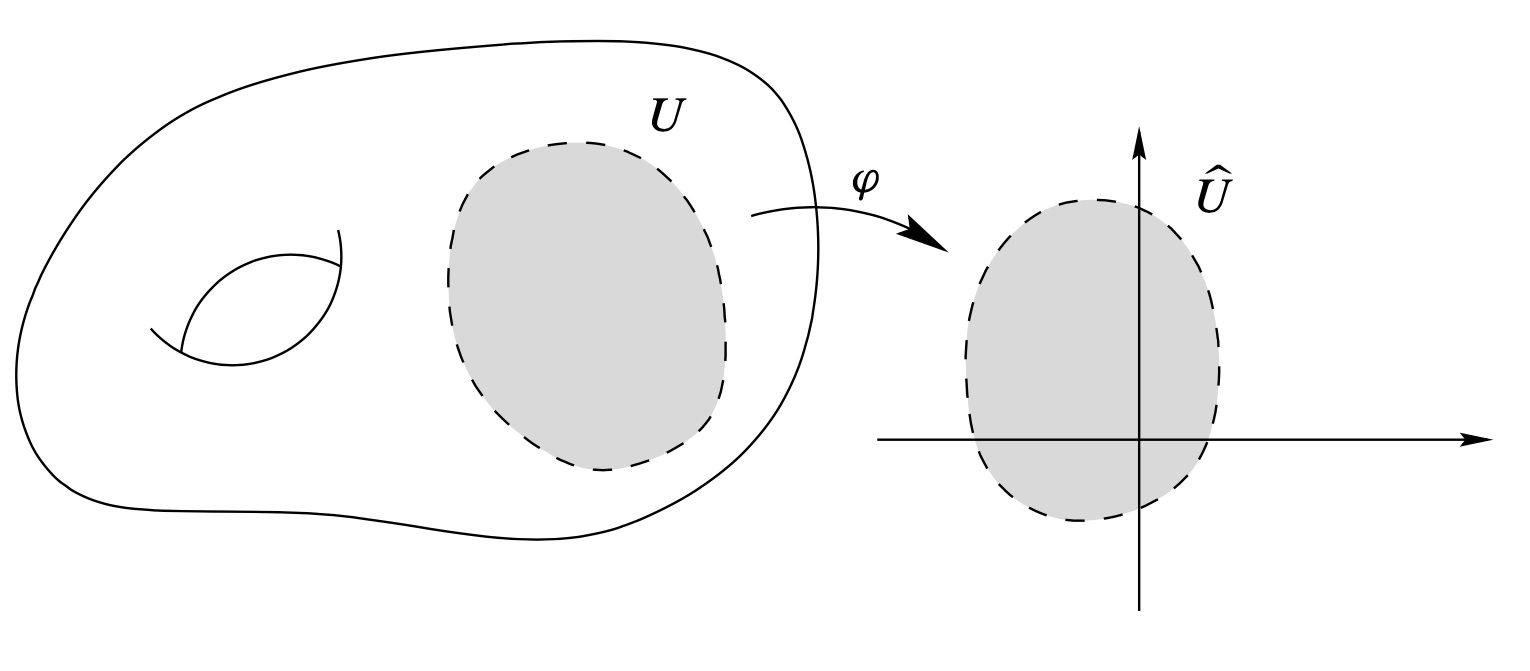
\includegraphics[width=12cm]{images/Lecture 2/Coordinate Chart.png} 
    \caption{\small{The visualization of a coordinate chart map from Lee's textbook on smooth manifolds \cite{Lee2012}}}
    \label{fig:Coordinate_Chart}
\end{figure}
\noindent If $(U, \phi)$, $(V, \psi)$ are two coordinate charts of a topological manifold $X$ and $U\cap V\neq\emptyset$, then $\psi \circ \phi^{-1} : \phi(U\cap V) \to \psi(U\cap V)$ is called a \textit{transition function} (see Fig. \ref{fig:Lee_TransitionMap}).
\begin{figure}
    \centering
    \captionsetup{format = hang}
    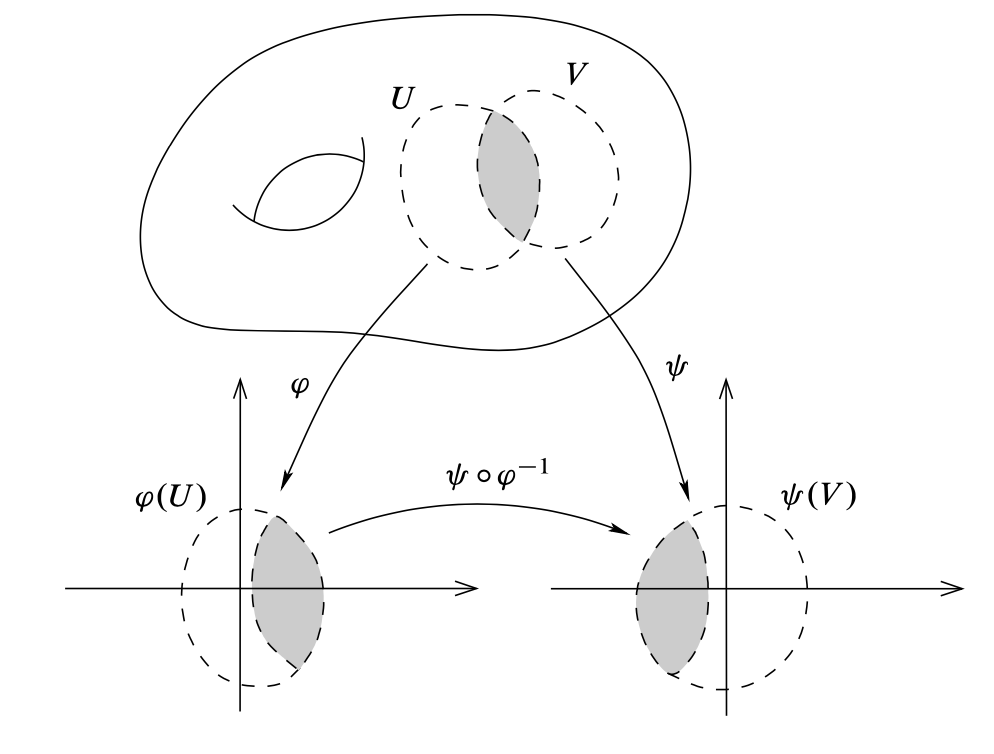
\includegraphics[width=12cm]{images/Lecture 2/Lee_TransitionMap .png} 
    \caption{\small{The picture of a transition function from \cite{Lee2012}}}
    \label{fig:Lee_TransitionMap}
\end{figure}

From the introduction it's clear that we will also deal with manifolds with boundary, so we recall also this definition. In order to do this we first introduce the following notation.
\begin{notat}[Half-space]
    By $\mathbb{H}^n$ we denote the $n$-dimensional upper (closed) half-space,
    $$\mathbb{H}^n=\{(x_1,...,x_n)\in\mathbb{R}^n|x_1 \leq 0\}$$ 
\end{notat}
\begin{defn}[Manifold with Boundary]
    A manifold with boundary of dimension $n$ is a paracompact (equivalently, second countable) Hausdorff topological space $X$ such that $X$ has an open cover $\{U_\alpha\}_\alpha$ together with a homeomorphism $\phi_\alpha:U_\alpha\to V_\alpha$ where $V_\alpha$ is an open subset of $\H^n$.\footnote{Note: a manifold with boundary, in general, is \textit{not} a manofold.}
\end{defn}
\begin{figure}
    \centering
    \captionsetup{format = hang}
    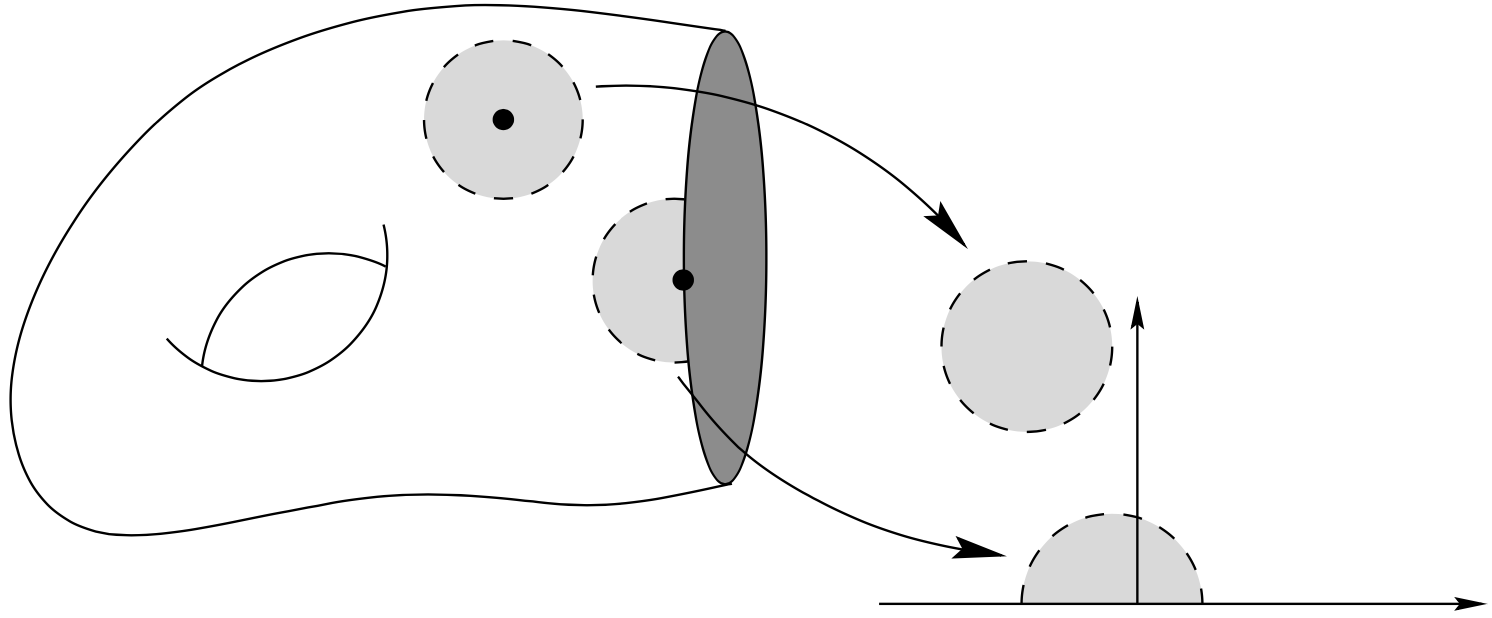
\includegraphics[width=12cm]{images/Lecture 2/Manifold with boundary.png} 
    \caption{\small{The picture of a 2-dimensional manifold with boundary from \cite{Lee2012}}}
    \label{fig:Manifold_w_boundary}
\end{figure}

\begin{defn}[Boundary of a Manifold]
    If for $p \in X$ and some chart $(U, \phi)$ it is the case that $x_i(\phi (p) )= 0$ (where $x_i:\R^n\to\R$ is the projection to the $i$-th coordinate), then it does in every chart\footnote{This is not trivial. If you know homology try to prove it.}. We then say that $p$ is in the \textit{boundary} of $X$, 
    $$
        \de X := \{ p \in X : x_i(p) = 0\}.
    $$
    otherwise, $p$ is in the \textit{interior} of $X$, which we denote with Int$(X)$ or $X^\circ$. 

    \noindent An equivalent definition is: $p \in \de X$ if $p$ has neighborhood $V$ that is the domain of a coordinate chart $\psi:V\to\H^n$ such that $\psi(V)\cap\de\H^n\neq\emptyset$ and sending $p$ to $\de \H^n$.
\end{defn}


\begin{lem}
    If $X$ is an $n$-dimensional manifold with boundary, then $\de X$ is a $(n-1)$-dimensional manifold.
\end{lem}
\begin{proof}
    Paracompactness and Hausdorff follow from being $\de X\subset X$ closed. Let $p\in\de X$ be an arbitrary point on the boundary of an $n$-manifold with boundary. Consider a chart containing $p$, $\phi:U\to V$. Since $p\in\de X$ we know that, w.l.o.g. $x_1(\phi(p))=0$ and $\phi(p)\in V\cap\de\mathbb{H}^n$. $\phi:U\to V$ can be restricted to a homemorphism $\phi\mid_{\phi^{-1}(V\cap\de\mathbb{H}^n)}:\phi^{-1}(V\cap\de\mathbb{H}^n)\xrightarrow{\cong}V\cap\de\mathbb{H}^n$. Note that $\phi^{-1}(V\cap\de\mathbb{H}^n)=U\cap\de X$. Note also that $\de\mathbb{H}^n\cong\R^{n-1}$. So $(U\cap\de X, \phi\mid_{U\cap\de X})$ is a chart around $p\in\de X$ into $\R^{n-1}$.
\end{proof}
\begin{defn}[Closed Manifold]
    A manifold is \textit{closed} if it is compact and without boundary, i.e. $\de X = \emptyset$. Conversely, an \textit{open} manifold is also a manifold without boundary but with no closed components, i.e. it has only non-compact components. 
\end{defn}

One can also do calculus on a manifold if some extra requirement are added to de definition of manifold. Before proceding in that, let us remind the reader of the following:
\begin{defn}[Smooth Function]
    Given $X\subseteq\R^n$ and $Y\subseteq\R^m$ a function $f:X\to Y$ is smooth\footnote{Also called infinitely differentiable or $C^\infty$.} if each of its component functions has continuous partial derivatives of all order.
\end{defn}

\begin{defn}[Smoothness in the Half Space]\label{SmoothHalf}
    If $X$ is an open subset of $\H^n$, we define $f:X\to\R^m$ to be smooth for each $x\in X$ if $X$ can be extended to an open subset $\tilde{X}\in\R^n$, and $f$ to a smooth map $\tilde{f}:\tilde{X}\to\R^m$ such that $\tilde{f}|_{\tilde{X}\cap\H^n}=f$. 
\end{defn}

\begin{defn}[Smooth Manifold Without Boundary]
    A smooth manifold with boundary $X$ is a topological manifold such that the transition functions $\phi_\beta\circ\phi^{-1}_\alpha$ are smooth in the sense of $\H^n$ (or $\R^n$ if $\de X=\emptyset$).
\end{defn}

\begin{ex}
    A lot of the spaces we think of can be equipped with a smooth manifold structure, such as:
    \begin{enumerate}
        \item the circle, a dimension $1$ manifold,
        \item genus $g$ surface, a dimension $2$ manifold,
        \item $\emptyset$, a smooth manifold of any dimension.
    \end{enumerate}
\end{ex}
\begin{notat}
    In these lecture notes, we will \textit{only} consider smooth manifolds, unless explicitly specified.
\end{notat}

\begin{cor}
    If $X$ is a \underline{smooth} $n$ dimensional manifold with boundary, then $\de X$ is a \underline{smooth} $(n-1)$ dimensional manifold.
\end{cor}
     
\begin{ex}% see how to go on another line for the first item. Solutions: \item[], \leavevmode, \hfill
\hfill 
\begin{enumerate}
    \item $D^n = \{x \in \R^n \mid  \ ||x||\leq 1\}$ the $n$ dimensional disk, which has a sphere as boundary: $\de D^n = S^{n-1}$
    \[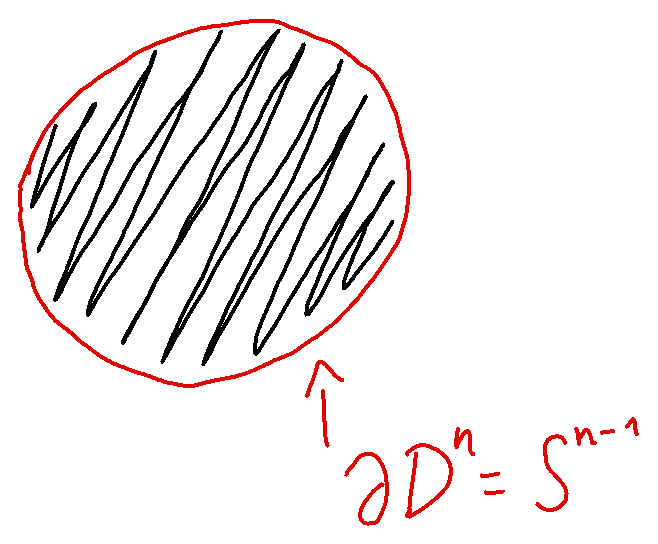
\includegraphics[width=5cm]{images/Lecture 2/Boundary Disk.png} \]
    \item Consider 2 dimensional \emph{open} disks, i.e. Int$(D^2)=\{x\in\R^2\mid \ ||x||<1\}$. Consider now the sphere $S^2$, if we then remove a number of open disks from if, we get the manifold $S^{2} \setminus\text{Int}(D^{2}_{1} \amalg D_2^2 \amalg D^2_3)$ which we can visualize in different ways.
    \[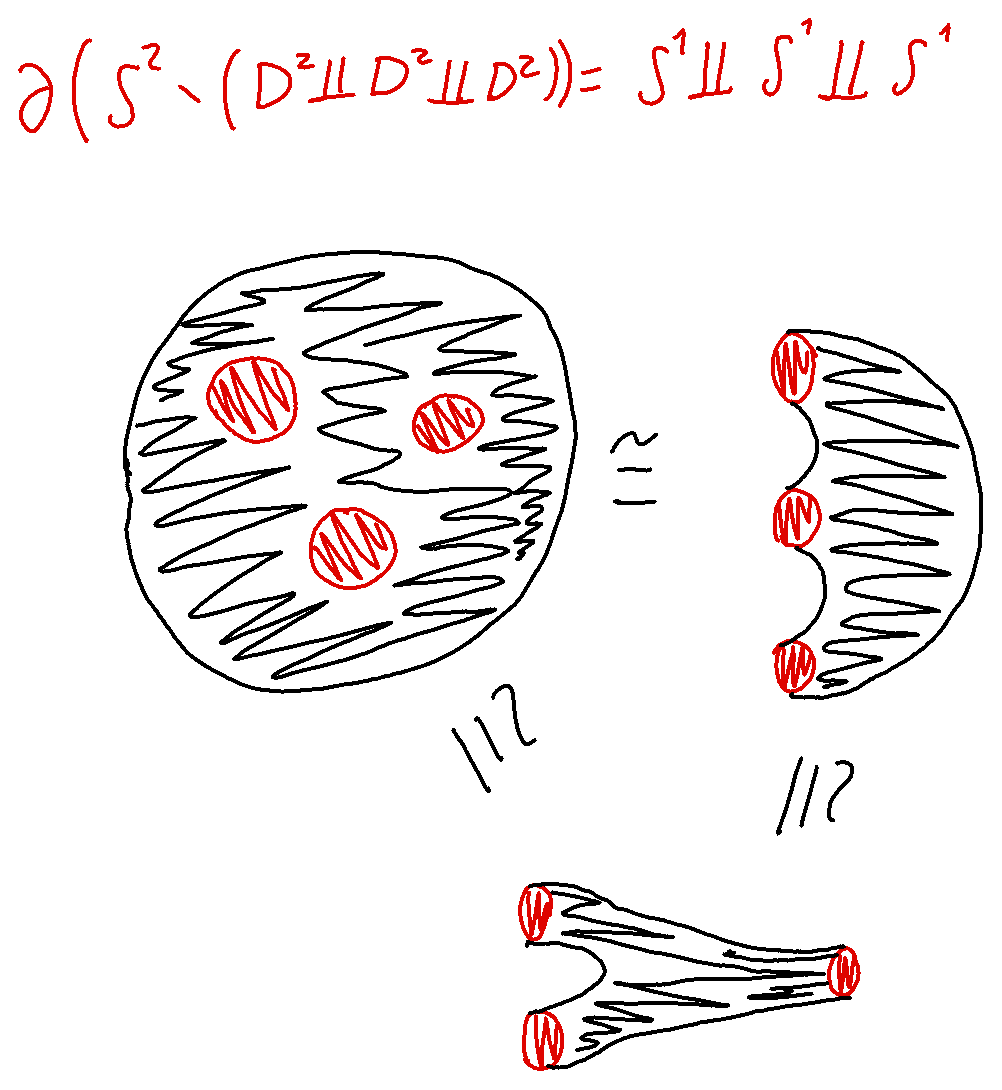
\includegraphics[width=7cm]{images/Lecture 2/Manifold3holes.png} \]
    \item Let $X, Y$ be $n$-manifolds with boundary, then $X \amalg Y$ is an $n$-manifold with boundary.
    \[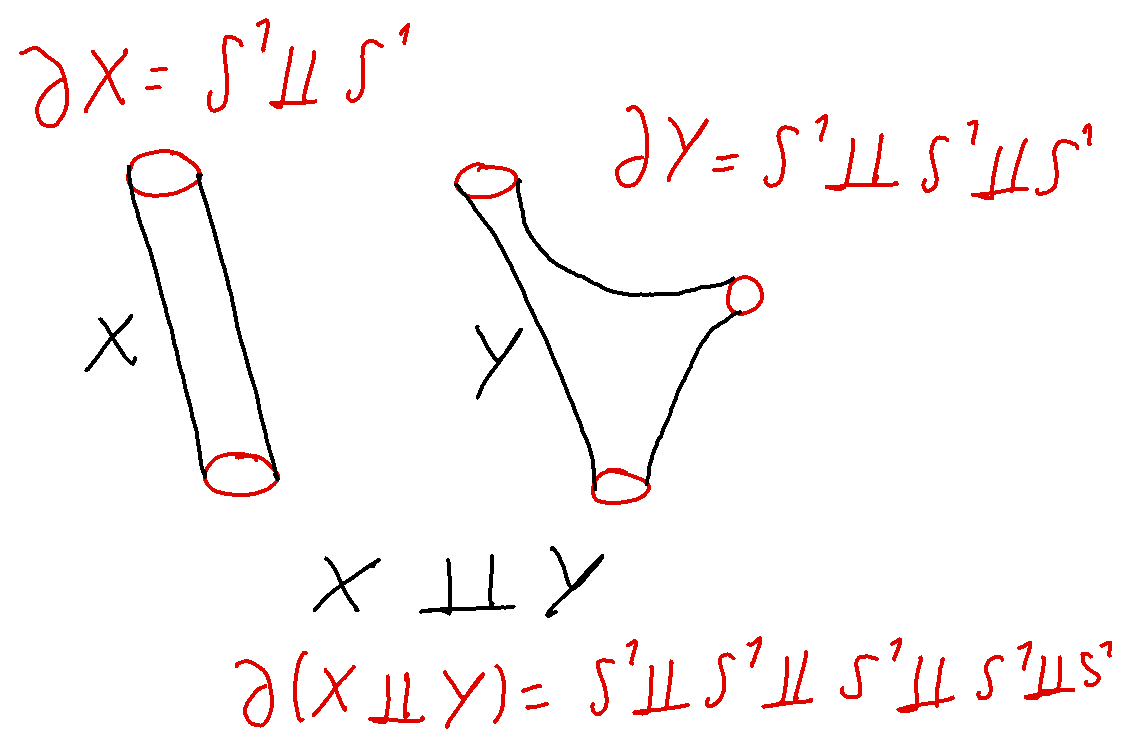
\includegraphics[width=7cm]{images/Lecture 2/Disjoint union of manifolds with boundary.png} \]
    \item $T= S^1 \times S^1$ is a $2$-manifold with $\de T = \emptyset$ and $T^{\text{solid}} = D^2 \times S^1$ is a $3$-manifold with $\de T^{\text{solid}} = T$.
        \[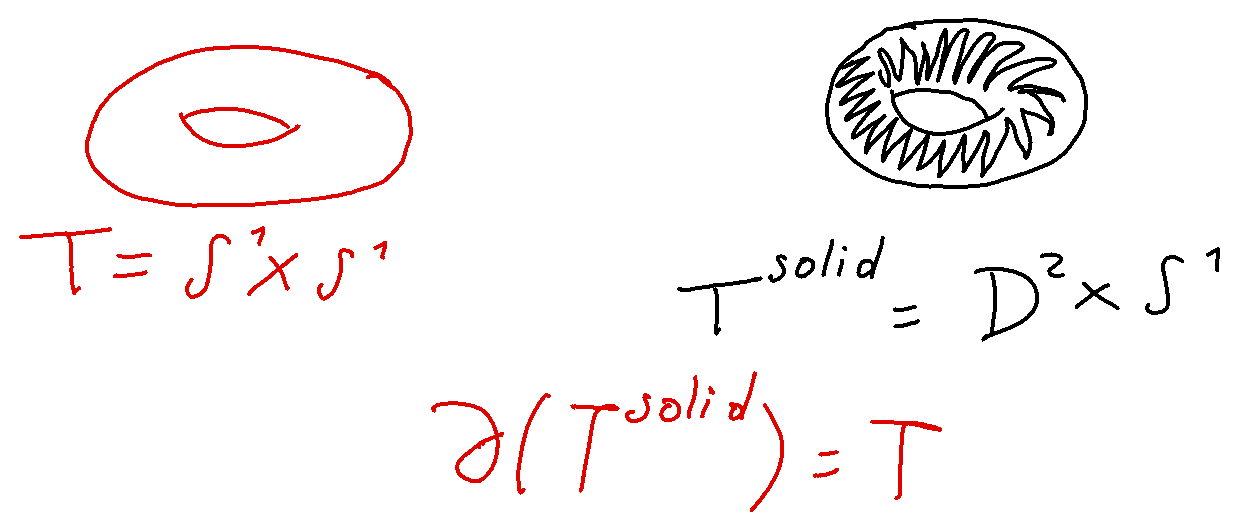
\includegraphics[width=7cm]{images/Lecture 2/Torus Boundary.png} \]
    \end{enumerate}
\end{ex}

\begin{defn}[Smooth Map on a Manifold]
    Let $X$ be a smooth manifold. $f:X\to\R^n$ is smooth if for each chart $(U,\phi)$ we have that $f\circ\phi^{-1}$ is smooth in the sense of $\R^n$.
\end{defn}

\noindent This definition can be generalized to maps between smooth manifolds.

\begin{defn}[Smooth Map between Manifolds]
    Let $X$ and $Y$ be smooth manifolds of dimensions $m$ and $n$ and $f:X\to Y$ a function between them. $f$ is smooth if for every $x\in X$ and chart $(U_x,\phi)$ containing $x$ and for a chart $(V_{f(x)},\psi)$ containing $f(x)\in Y$ then$\tilde f = \psi \circ f\circ \phi^{-1}$ is smooth. This can be represented in the following diagram:
    \begin{equation*}
        \begin{tikzcd}
            {X\supseteq U} &&& {V\subseteq Y} \\
            &&& {} \\
            {\mathbb{H}^m\supseteq\tilde{U}} &&& {\tilde{V}\subseteq\mathbb{H}^n}
            \arrow["f|_U", from=1-1, to=1-4]
            \arrow["{\psi_x}", from=1-4, to=3-4]
            \arrow["{\tilde{f}}"', from=3-1, to=3-4]
            \arrow["\cong"', from=1-4, to=3-4]
            \arrow["{\phi_x}"', from=1-1, to=3-1]
            \arrow["\cong", from=1-1, to=3-1]
        \end{tikzcd}
    \end{equation*}
\end{defn}
\noindent Is this notion well defined? Or, in other words, is it possible that a function is smooth in one chart and not another? No! Check this.
\begin{defn}[Diffeomorphism of Manifolds]
    A diffeomorphism is a smooth map with a smooth inverse. This, we will see, defines the notion of an isomorphism in the \textit{category of smooth manifolds}.
\end{defn}

\begin{exercise}
    Come up with the natural notion of smooth map between manifolds \emph{with} boundary. 
\end{exercise}

\section{What is a bordism?}

The idea of a bordism is to identify (and maybe classify) manifolds that ``differ'' by a manifold. A first definition, that will turn out to be too strict, is the following.
\begin{defn}[$1^{st}$ variant of the definition of bordism: via \emph{strict equalities}]
\label{Define Bordism}
    Let $Y_0, Y_1$ be closed $n$-manifolds. A bordism $(X,p)$ from $Y_0$ to $Y_1$ consists of a compact $(n+1)$-manifold with boundary together with a map $p: \de X \to \{0,1\}$ such that $Y_0 = p^{-1}(0)$ and $Y_1 = p^{-1}(1)$. Thus, $\de X = Y_0 \amalg Y_1$.

    \noindent We then say that $Y_0$ and $Y_1$ are \textit{cobordant}.
\end{defn}
\noindent We call $Y_0$ the \textit{incoming} boundary and $Y_1$ the \textit{outgoing} boundary. We sometimes write $\de_{in} X = Y_0$ and $\de_{out} X = Y_1$.

\begin{ex}
    ``pair of pants'' %DRAWING
    \begin{figure}[!ht]
        \centering
        \captionsetup{labelformat=empty, format = hang}
        \begin{measuredfigure}
            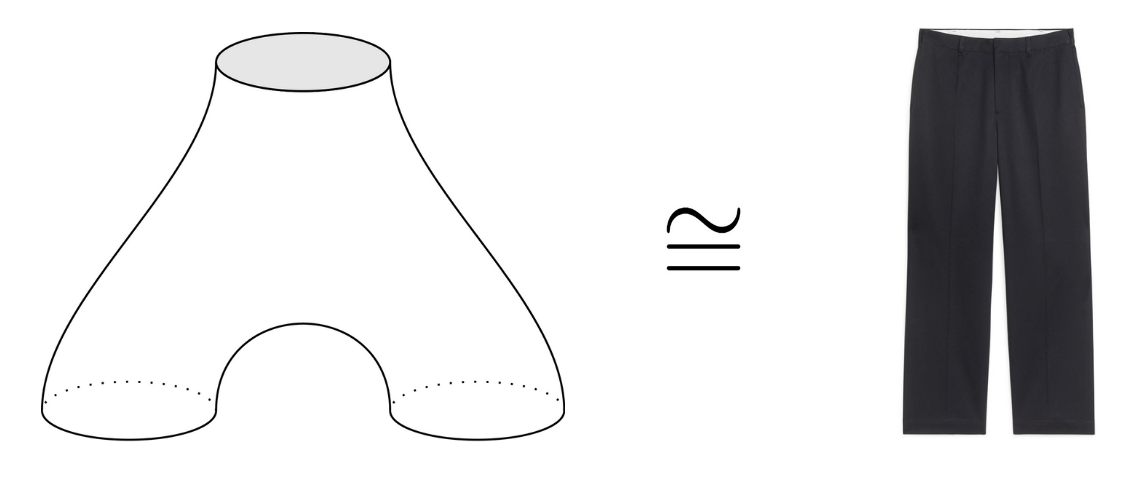
\includegraphics[width=9cm]{images/Lecture 2/pants_topological.png} 
            \caption{\small{Bordism from $S^1$ to $S^1\amalg S^1$}}
        \end{measuredfigure}
    \end{figure}
\end{ex}

\begin{ex} 
\hfill
\begin{itemize}
    \item The torus is a bordism from $\emptyset$ to $\emptyset$. ($\de T = \emptyset = Y_0 \amalg Y_1 \implies Y_0 = Y_1 = \emptyset$)
    %\begin{figure}[!ht] % Torus as a bordism: empty -> empty
        %\centering
    \begin{center} % changed it to this so the picture is exactly here
        \begin{tikzpicture}
            \node (A) at (-3,0) {};
            \node (B) at (-3,-2){\small{$Y_0 = \emptyset$}};
            \draw[->] (A)--node[auto, align=center]{}(B);
            
            \pic{torus={2cm}{5.6mm}{70}};

            \node (C) at (3,0) {};
            \node (D) at (3,-2){\small{$Y_1 = \emptyset$}};
            \draw[->] (C)--node[auto, align=center]{}(D);
        \end{tikzpicture}
    \end{center}
    %\end{figure}\vspace{-6mm}
    %
    \item   $X = S^1 \times [0,1]$, now $\de X = S_1 \amalg S_1$ and we can view it as a bordism in 4 ways:
    \begin{figure}[H]
    \centering
    \begin{subfigure}[t]{.4\textwidth}
        \centering
        \begin{tikzpicture}[scale=0.8]
            \tikzmath{\cylH = 3; \cylr = 0.5; \cylR = 1.25; \spc = 0.75;} 
            \node (A) at (-\spc, 0) {};
            \node (B) at (-\spc, -\cylR - \spc){\scriptsize{$Y_0 = S^1\times\{0\}$}};
            \draw[->] (A)--node[auto, align=center]{}(B);
            
            \draw (0, 0) ellipse ({\cylr} and {\cylR});
            \draw (0, \cylR) -- (\cylH, \cylR);
            \draw (0, -\cylR) -- (\cylH, -\cylR);
            \draw [dashed] (\cylH, \cylR) arc (90:270:{\cylr} and {\cylR});
            \draw (\cylH,\cylR) arc (90:270:{-\cylr} and {\cylR});

            \node (C) at (\cylH + \spc, 0) {};
            \node (D) at (\cylH + \spc, -\cylR - \spc){\scriptsize{$Y_1 = S^1\times\{1\}$}};
            \draw[->] (C)--node[auto, align=center]{}(D);
        \end{tikzpicture}
    \end{subfigure}
    \hspace{5mm}
    \begin{subfigure}[t]{.4\textwidth}
        \centering
        \begin{tikzpicture}[scale=0.8]
                \tikzmath{\cylH = 3; \cylr = 0.5; \cylR = 1.25; \spc = 0.75;} 
                \node (A) at (-\spc, 0) {};
                \node (B) at (-\spc, -\cylR - \spc){\scriptsize{$Y_0 = S^1\times\{1\}$}};
                \draw[->] (A)--node[auto, align=center]{}(B);
                
                \draw (0, 0) ellipse ({\cylr} and {\cylR});
                \draw (0, \cylR) -- (\cylH, \cylR);
                \draw (0, -\cylR) -- (\cylH, -\cylR);
                \draw [dashed] (\cylH, \cylR) arc (90:270:{\cylr} and {\cylR});
                \draw (\cylH,\cylR) arc (90:270:{-\cylr} and {\cylR});
    
                \node (C) at (\cylH + \spc, 0) {};
                \node (D) at (\cylH + \spc, -\cylR - \spc){\scriptsize{$Y_1 = S^1\times\{0\}$}};
                \draw[->] (C)--node[auto, align=center]{}(D);
        \end{tikzpicture}
    \end{subfigure}

    \medskip
        
    \begin{subfigure}[t]{.4\textwidth}
        \centering
        \begin{tikzpicture}[scale=0.8]
            \tikzmath{\cylH = 3; \cylr = 0.25; \cylR = 0.75; \spc = 0.6; \gp = 0.5;} 
            \node (A) at (-\spc, -\cylR - \gp/2) {};
            \node (B) at (-\spc, -3 * \cylR - \gp -\spc){\scriptsize{$Y_0 = S^1\amalg S^1$}};
            \draw[->] (A)--node[auto, align=center]{}(B);
            
            \draw (0, 0) ellipse ({\cylr} and {\cylR});
            \draw (0, -2 * \cylR - \gp) ellipse ({\cylr} and {\cylR});
            
            \draw (0,-\cylR) arc (90:270:{-1.5*\cylr} and {\cylr});
            \draw (0,\cylR) arc (90:270:{-2*\cylR} and {2*\cylR + \gp/2});
    
            \node (C) at (2*\cylR + \spc/2, -\cylR - \gp/2) {};
            \node (D) at (2*\cylR + \spc/2, -3 * \cylR - \gp -\spc){\scriptsize{$Y_1 = \emptyset$}};
            \draw[->] (C)--node[auto, align=center]{}(D);
        \end{tikzpicture}\hspace{10mm}
    \end{subfigure}
    \begin{subfigure}[t]{.4\textwidth}
        \centering
        \begin{tikzpicture}[scale=0.8]
            \tikzmath{\cylH = 3; \cylr = 0.25; \cylR = 0.75; \spc = 0.6; \gp = 0.5;} 
            \node (A) at (-\spc / 2, -\cylR - \gp/2) {};
            \node (B) at (-\spc / 2, -3 * \cylR - \gp -\spc){\scriptsize{$Y_0 = \emptyset$}};
            \draw[->] (A)--node[auto, align=center]{}(B);
            
            \draw (2*\cylR, 0) ellipse ({\cylr} and {\cylR});
            \draw (2*\cylR, -2 * \cylR - \gp) ellipse ({\cylr} and {\cylR});
            
            \draw (2*\cylR,-\cylR) arc (90:270:{1.5*\cylr} and {\cylr});
            \draw (2*\cylR,\cylR) arc (90:270:{2*\cylR} and {2*\cylR + \gp/2});

            \node (C) at (2*\cylR + \spc, -\cylR - \gp/2) {};
            \node (D) at (2*\cylR + \spc, -3 * \cylR - \gp -\spc){\scriptsize{$Y_1 = S^1\amalg S^1$}};
            \draw[->] (C)--node[auto, align=center]{}(D);
        \end{tikzpicture}
    \end{subfigure}
    \end{figure}
    The latter two are sometimes calles ``macaroni''.
    
    This shows that different bordisms can arise from the same underlying manifold. We will have a way of differentiating them when we will introduce tangential structures on a manifold, which will enable us to explain in which direction a manifold is oriented.

    \item Given two $n$-manifolds $M,N$, their \textit{connected sum} is 
    \begin{equation*}
         M\# N=M\setminus(D^{n})^{\circ}\coprod_{S^{n-1}} N\setminus(D^{n})^{\circ}
     \end{equation*}
     where ${}^{\circ}$ is for taking the interior and $\coprod_{S^{n-1}}$ is glueing along the new boundaries in $N$ and $M$.
    \begin{figure}[!ht]
    \centering
    \captionsetup{labelformat=empty, format = hang}
        \begin{measuredfigure}
            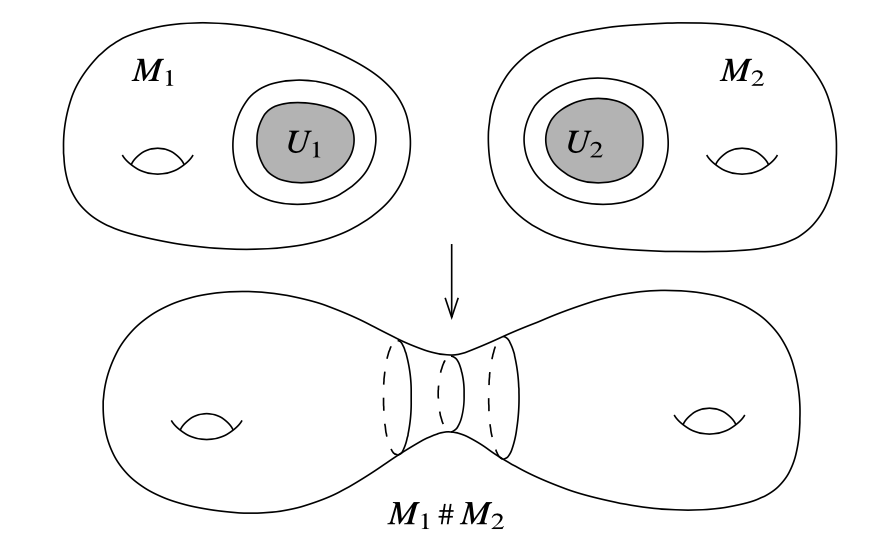
\includegraphics[width=9cm]{images/Lecture 2/connected sum.png} \caption{\small{The picture of a connected sum from \href{https://en.wikipedia.org/wiki/Connected_sum]}{Wikipedia}}}
        \end{measuredfigure}
    \end{figure}
\end{itemize}
\end{ex}
\begin{prop}
    $M\# N$ is an $n$-manifold.
\end{prop}
%proof to be added?
\begin{lem}
    There is a bordism between $M\coprod N$ and $M\# N$.
\end{lem}

\begin{proof} 
    A bordism between $M_1\coprod M_2$ and $M_1\#M_2$ may be constructed in the following manner (proof taken from the \href{http://www.map.mpim-bonn.mpg.de/Bordism#Connected_sum_and_bordism}{Manifold Atlas Project}). Consider a cylinder $M_1\times I$, from which we remove an $\epsilon$-neighbourhood $U_{\epsilon}(v_{1}\times 1)$ of the point $v_{1}\times 1$. Similarly, remove the neighbourhood $U_{\epsilon}(v_{2}\times 1)$ from $M_{2}\times I$ (each of these two neighbourhoods can be identified with the half of a standard open $(n+1)$-ball). Now connect the two remainders of cylinders by a "half pipe" $\left(S_{n}\leq 0 \right)\times I$ in such a way that the half-sphere $S_{n}\leq 0$ is identified with the half-sphere on the boundary of $U_{\epsilon}(v_{1}\times 1)$, and $\left(S_{n}\leq 0 \right)\times I$ is identified with the half-sphere on the boundary of $U_{\epsilon}(v_{2}\times 1)$. Smoothening the angles we obtain a manifold with boundary $(M_1\coprod M_2)\coprod(M_1\#M_2)$.
\begin{figure}[H]
\centering
\captionsetup{labelformat=empty, format = hang}
    \begin{measuredfigure}
        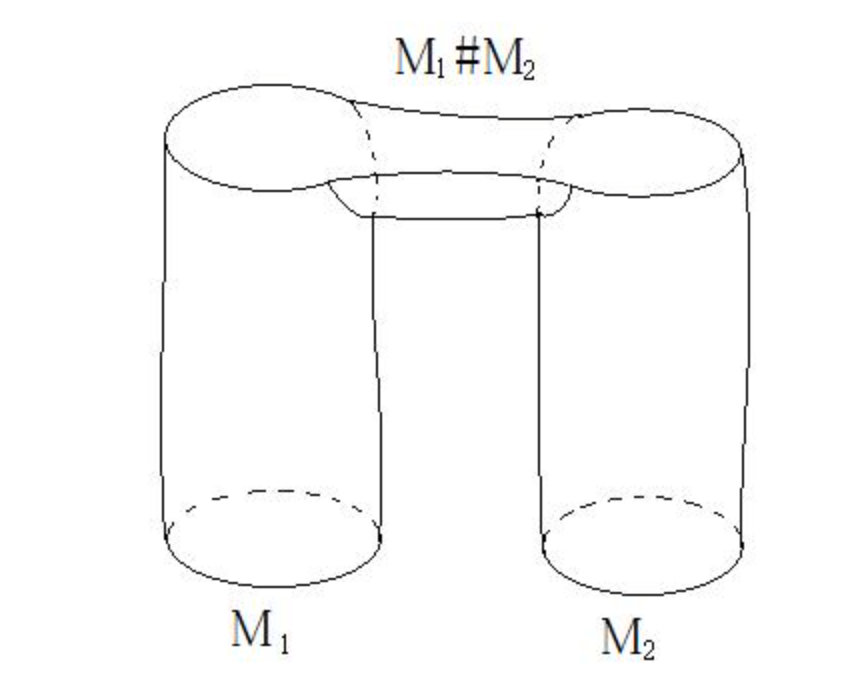
\includegraphics[width=6cm]{images/Lecture 2/Bordism connected sum to disjoint union.png} 
        \caption{\small{The illustration by the \href{http://www.map.mpim-bonn.mpg.de/Bordism\#Connected_sum_and_bordism}{Manifold Atlas Project} of the bordism constructed in the proof above}}
    \end{measuredfigure}
\end{figure}
\end{proof}
%add Drawings inspired by the Prof.'s examples?
\begin{thm}
\label{Cobordant Equiv}
Being cobordant is an equivalence relation on closed $n$-manifolds. 
\end{thm}
\begin{proof}
We need to show that the relation satisfies the properties of reflexivity, symmetry and transitivity:
\begin{itemize}
    \item Reflexive: $Y_0 \sim Y_0$ since we can take $X = Y_0 \times [0,1]$ as in the previous example. We then have $\de X = Y_0 \times \{0,1\} \xrightarrow{p} \{0,1\}$. 
    %
    \item Symmetric: assume $Y_0 \sim Y_1$. Thus, we have $(X,p)$ from $Y_0$ to $Y_1$. We can use the same manifold and compose $p$ with the $swap$ of 0 and 1 in order to get 
    $$\tilde{p}=(swap) \circ p:\de X\xrightarrow{p}\{0,1\}\xrightarrow{swap}\{1,0\}$$ Consequently, $(X, swap \circ p)$ is a bordism from $Y_1$ to $Y_0$.
    %
    \item Transitive: we have $Y_0 \sim Y_1$ via $(X_1, p_1)$ and $Y_1 \sim Y_2$ via $(X_2, p_2)$. 
    Then we can use as a manifold $X = X_1 \cup_{Y_1} X_2$ where $\cup_{Y_1}$ indicates the gluing along $Y_1$. 
    This is a manifold but there's some work involved in showing it's a \textit{smooth} manifold and it will be done later 
    on (\ref{BordantTransitive}), via an equivalent definition of bordism. We then think of the boundary in the following
     way $\de X = \de_{in} X_1 \amalg \de_{out} X_2$.
\end{itemize}
\end{proof}

% -------------------------------------------------------------
% --------------------- LECTURE 3 30/10 -----------------------
% -------------------------------------------------------------
\section{Different definitions of bordisms} % (fold)
\label{sec:different_definitions_of_bordisms}

\begin{rmnd}[Definition \ref{Define Bordism} of Bordism]
Let $Y_0, Y_1$ be closed $n$-manifolds. A bordism $(X,p)$ from $Y_0$ to $Y_1$ consists of a compact $(n+1)$-manifold with boundary together with a map $p: \de X \to \{0,1\}$ such that $Y_0 \text{\colorbox{yellow}{=}} p^{-1}(0)$ and $Y_1 \text{\colorbox{yellow}{=}} p^{-1}(1)$ (hence $\de X \text{\colorbox{yellow}{=}}  Y_0 \amalg Y_1$). We say that $Y_0$ and $Y_1$ are \textit{cobordant}.
\end{rmnd}

\noindent There was a complaint: why don't we use diffeomorphisms instead of the highlighted equalities? This question arises because even with simple examples the equality seems too strict:

\begin{rmnd}[from \ref{Cobordant Equiv}]
Being cobordant is an equivalence relation.
\end{rmnd} 

\noindent In particular, for any closed $n$-manifold $Y$ we have $Y\sim Y$. The bordism is given by the cylinder $Y\times [0,1]$, where $p:Y\times\{0,1\}\to \{0,1\}$. Then $Y\times\{0\}=p^{-1}(0)$, but $Y\neq Y\times\{0\}$! 
It seems like our previous definition does not actually give rise to an equivalence relation. 
%TODO is this above what we wanted to say? /William
Instead, if we substitute the strict equalities with diffeomorphisms (isomorphisms in the category of smooth manifolds) things seem to work out flawlessly:

\begin{defn}[$2^{nd}$ variant of the definition of bordism: via diffeomorphisms]
\label{NewDefBord}
    Let $Y_0, Y_1$ be closed $n$-manifolds. A bordism from $Y_0$ to $Y_1$ is a quadruple $(X,p,\phi_{0},\phi_{1})$ consisting of a compact $(n+1)$-manifold with boundary $\de X$ together with maps 
    \begin{align*}
        p&: \de X \to \{0,1\}        \\
        \phi_{0}&:Y_{0}\xrightarrow{\cong} p^{-1}(0) \\
        \phi_{1}&:Y_{1}\xrightarrow{\cong} p^{-1}(1)
    \end{align*}
    (we therefore have $\de X \cong Y_0 \amalg Y_1$).
\end{defn}

\begin{ex}
    Let $\psi:M\xrightarrow{\cong} N$ be a diffeomorphism.
    Then $(M\times [0,1], M\times\{0,1\}\xrightarrow{p}\{0,1\}, \phi_0, \phi_1)$, with maps
    $$\phi_0:M\xrightarrow{id\times\{0\}}p^{-1}(0)=M\times \{0\}$$
    $$\phi_1:N\xrightarrow{\psi^{-1}\times\{1\}}p^{-1}(1)=M\times\{1\}$$
    gives a bordism from $M$ to $N$.
    This is called the mapping cylinder of $\psi$. 
    
    \noindent$\Rightarrow$ under the new definition, \underbar{any} two diffeomorphic manifolds are also cobordant.
\end{ex}

%TODO it's not really clear what the mapping cylinder is

Why does this not change the definition of bordism?
Because any diffeomorphism also gives a bordism in the old sense:
Given $M\xrightarrow{\cong}N$, take the gluing $(M\times I)\underset{M\times\{1\}}{\coprod_{\psi}}N$ so that $Y_1=N$ and $Y_0=M\times \{0\}"="M$ (abusing notation).

\noindent Now we prove the transitivity of the relation 'being cobordant'. We do that by showing that given $X$ from $Y_0$ to $Y_1$ and $X'$ from $Y_1$ to $Y_2$, we can glue them along the boundary in common, $Y_1$, to obtain a bordism from $Y_0$ to $Y_2$. %add diagram here (?) later works as well
In order to achieve this, we need to introduce the following notion:
\begin{defn}[Collar of a boundary]
    Let $X$ be a manifold with boundary. A collar of the boundary is an open set  $U\subseteq X$ containing $\de X$ together with a diffeomorphism  $(-\epsilon,0]\times\partial M \to U$ for some $\epsilon>0$.
\end{defn}
\begin{thm}
    The boundary of a manifold with boundary always has a collar.
\end{thm}
\begin{proof}[Idea of the proof]
    We start with a manifold with boundary, locally at $x\in\de X$ we have 
    $$(-\epsilon_x, 0]\times V_x\xrightarrow{\cong} U_x\subseteq\mathbb{H}^n$$
    where $V_x$ is an open neighbourhood of $x$ in $\de X$.
    \noindent Now we use a standard trick in differential geometry/topology (see \cite{Hirsch1976}): globally patch these diffemorphisms using a partition of unity. It works if $X$ is compact.
\end{proof}

\begin{defn}[$3^{rd}$ variant of the definition of bordism: via collars]
    Let $Y_0$ and $Y_1$ be closed $n$-manifolds. A bordism from $Y_0$ to $Y_1$ is a quadruple $(M, p, \phi_0, \phi_1)$ with $M$ and $p$ as before. $\phi_0, \phi_1$ are given by
    $$\phi_0:[0, \epsilon)\times Y_0\to U \supseteq p^{-1}(0)$$
    $$\phi_1:(-\epsilon, 0]\times Y_1\to V \supseteq p^{-1}(1)$$
    where $U$ and $V$ together form a collar of the boundary of $M$.
\end{defn}

\noindent Moreover, 
$$([0, \epsilon)\times Y_0\big)\amalg((-\epsilon, 0]\times Y_1)\xrightarrow{\phi_0\amalg\phi_1}
\big(U\amalg V\big)\supseteq 
\Big(p^{-1}(0)\amalg p^{-1}(1)\Big)=\de M$$
%TODO what is this for?

\noindent This variant of the definition is equivalent to the other two but we would unfortunately need a lot of differential topology in order to prove this.

However, with the third definition we can finally prove the following claim which then is what we were missing to prove transitivity of being cobordant.
\begin{clm}\label{GluedManifoldsBordisms}
    $X\underset{Y_1}{\cup} X'$ admits a smooth structure.
\end{clm}
\begin{proof}[Transitivity of cobordant]\label{BordantTransitive}
    We need a maximal atlas with smooth transition functions. Clearly, in the interior points of $X$ and $X'$ this exists since we can use directly the charts of $X$ and $X'$. The problem is the double collar around $Y_1$. So we need to construct charts around points on $Y_1$. Take $U_1^{-}\underset{Y_1}{\cup}U_1^{+}$ in an open neigbourhood. Then via $U_1^{-}\underset{Y_1}{\cup}U_1^{+}\xrightarrow{\phi_1\cup\phi'_0}(-\epsilon,\epsilon)\times Y_0=(-\epsilon,0]\cup[0,\epsilon)\times Y_0$ which contains $(-\epsilon,\epsilon)\times V_x$ which maps to $\R^n$ via $\psi_x$ and thereby generating a maximal atlas.

%TODO not very clear
Let $X$ be a bordism between $Y_0$ to $Y_1$ and $X'$ between $Y_1$ and $Y_0$.
%drawings
$$[0, \epsilon)\times Y_0\xrightarrow{\phi_0}U$$
$$(-\epsilon,0]\times Y_1\xrightarrow{\phi_1}U_1^{-}$$
$$[0,\epsilon)\times Y_1\xrightarrow{\cong}(-\epsilon,0]\times Y_1\xrightarrow{\phi'_0}U_1^{+}$$
$$(-\epsilon,0]\times Y_2\xrightarrow{\phi'_1}U_2$$
\end{proof}

\section{Tangential Structures}
\subsection{Orientations and the tangent bundle}
\begin{defn}[Tangent bundle]
    The tangent bundle $TM$ of a bundle $M$ is the vector bundle over $M$ of rank $n$ with
    \begin{enumerate}
        \item fibers given by the tangent spaces $T_p M$ at each point $p \in M$: $$(TM)_p=T_pM$$
        \item (as a set) $TM=\coprod_{p\in M} T_p M$ with natural projection: 
        \begin{align}
            TM=\coprod_{p\in M} T_p M&\xrightarrow{p}M \\
            (p,v)&\mapsto p
        \end{align}
    \end{enumerate}
\end{defn}

\noindent It is possible to define a topology on $TM$ such that it is a smooth $2n$ manifold: $(U,\phi)$ chart of $M$, we have a chart of $TM$, $(p^{-1}(U),\tilde\phi)$ by looking at preimages of $U$ under the projection map and we construct the local trivialization with the usual construction. 
%TODO maybe say a bit more about local trivialisations
This is summarized by the fact that the following diagram commutes:
\[\begin{tikzcd}
    {p^{-1}(U)=TU=\coprod_{p\in U}T_pM} && {T\tilde U=\tilde U\times\R^n} \\
    \\
    U && {\tilde U\subseteq\R^n}
    \arrow["p", from=1-1, to=3-1]
    \arrow["{\tilde\phi=(\phi,d\phi)}"', from=1-1, to=1-3]
    \arrow["pr_{\tilde U}", from=1-3, to=3-3]
    \arrow["\phi"', from=3-1, to=3-3]
    \arrow["\cong", from=3-1, to=3-3]
\end{tikzcd}\]
This is actually an atlas with smooth structure. Transition functions $g_{ij} = \tilde \phi_j \circ \tilde\phi_i^{-1}|_{\tilde \phi_i(U_i \cap U_j)}$ are actually the jacobian and we have $g_{ij} \in GL_n(\R)$. 

\begin{defn}[Orientability and admissibility of $G$ structure]
    If $TM$ has local trivializations such that the transition functions between overlapping trivializations are in $ GL_n^+(\R)\subseteq GL_n(\R)$ then we say that $M$ is orientable.

    \noindent In other words ``''The structure group of $TM$ can be reduced to $GL_n^+ (\R) \subset GL_n(\R)$''.
    
    \noindent Analogously, given some $G \subset GL_n(\R)$, we can say $M$ admits a $G$ structure if the local trivialisations are such that $\phi_{i,j} \in G$, i.e. "the structure group can be reduced to $G$". In this sense, being orientable is the same as admitting a $GL_n^+ (\R)$ structure.

\end{defn}

% -------------------------------------------------------------
% --------------------- LECTURE 4 6/11 -----------------------
% -------------------------------------------------------------

\begin{ex}
\hfill
    \begin{itemize}
        \item $\R^n$: we have $T\R^n \cong \R^n \times \R^n$, meaning the tangent bundle is a trivial bundle.
        \item $S^1$: we again have the trivial bundle $TS^1 \cong S^1 \times \R$
        \item $S^2$: now $TS^2 \ncong S^2 \times \R^2$, it is not a trivial bundle. This follows from the \href{https://en.wikipedia.org/wiki/Hairy_ball_theorem}{hairy ball theorem}. 
    \end{itemize}
    All these are orientable. Instead examples of non orientable manifolds are the Klein bottle, the Möbius strip and $\R\P^2$.
 %drawings 
\end{ex}

\begin{defn}[Orientation and $G$ structure]
    An orientation (equivalently, a $GL^+_n(\R)$ structure) of $M$ is an equivalence class of trivialisations $\{(\tilde U, \tilde \phi)\}$ of $TM$ such that $\det g_{ij} > 0$ (i.e. $g_{ij} \in GL^+(n,\R)$).

    \noindent Analogously, given some $G \subset GL_n(\R)$, a $G$ structure on $TM$ is an equivalence class of trivialisations $\{(\tilde U, \tilde \phi)\}$ such that $g_{ij} \in G$.
\end{defn}

\noindent We can now note the following lemma which is related to the fact that on a manifold one can always construct a Riemannian metric.
\begin{lem}
    A $GL_n^+ (\R)$ structure is the same as an $SO(n)$ structure.
\end{lem}

\noindent How many orientations can $M$ have? $0$ if it's not orientable, $2$ if it's connected and orientable, in general $2^{\# \text{ connected components}}$ if it's orientable.

\begin{defn}[Opposite orientation]
    $M$ oriented with charts $\{(U_i, \phi_i)\}$. The opposite orientation on $M$ is given by: $\{(U_i, \bar \phi_i)\}$ in which $\bar \phi_i$ is given by the following composition
    \begin{equation}
        U_i \xrightarrow{\phi_i} \R^n \xrightarrow{ \ x_1\mapsto-x_1 \ } \R^n %TODO write better
    \end{equation}
    We will indicate $M$ with opposite orientation by $\bbar M$.
\end{defn}

\begin{ex}
    $S^1$ %DRAWING
\end{ex}
Note that a diffeomorphism between two orientable manifolds can induce orientations: if we have $f:M\to N$ and choose an orientation on $M$ i.e. a proper choice of trivialization $(U_\alpha, \phi_\alpha)$, then on $N$ we can define a trivialization $(V_\alpha,\psi_\alpha)$ with $V_\alpha:=f(U_\alpha)$ and $\psi_\alpha:=\phi_\alpha\circ f^{-1}$. First note that, being $f$ a diffeomorphism, everything in perfectly well defined. Then note: $\psi_\alpha\circ\psi_\beta^{-1}=(\phi_\alpha\circ f^{-1})\circ (f\circ \phi_\beta^{-1})=\phi_\alpha\circ\phi_{\beta}^{-1}$ and thus the determinand of the transition functions on $N$ is the same as the ones of $M$!
\begin{defn}[Orientation preserving and reversing diffeomorphism]
    A diffeomorphism $f: M \to N$ between oriented manifolds is orientation preserving (reversing) if the orientation on $N$ induced by the one on $M$ is the (opposite) orientation on $N$ $\iff \text{det}(df_p)>0$ (or $<0$) for all $p\in M$.
\end{defn}
\begin{ex}
    Consider maps $S^1 \to S^1$ (implicitly using the same orientation on each $S^1$). The identity is an orientation preserving map, while the map $x \mapsto \bar x$ is orientation reversing (considering $S^1 \subset \C$).

    \noindent We could instead consider maps $S^1 \to \bbar{S^1}$. In this case the identity is orientation reversing.
\end{ex}

Consider a oriented manidold $M$ with boundary. By a previous theorem we know that $\de M$ is a manifold itself and thus we can talk of it's tangent bundle $T\de M$. At the same time, we can ``glue another collar'' $[0,\epsilon)$ onto the boundary so that the points of the boundary are now in the interior of the new extended manifold thus allowing us to define the tangent space $T_p M$ for $p\in \de M$ (this construction is independent from the extension). Now, we can consider $T\de M$ as a subspace of $TM|_{\de M}$ via the inclusion $i: \de M \to M$ which induces $i_*: T(\de M)\to TM$.
%DRAWING
We can then define the quotient
$$
    \nu_p = T_p M /i_*T_p \de M \cong \R
$$
and we can write the following short exact sequence of bundles on $\de M$.
\begin{equation}
    0 \to i_*T(\de M) \to TM \to \nu \to 0
\end{equation}
This is saying that the tangent bundle over $M$ on a boudary point is the tangent bundle of the boundary plus an extra ``normal'' direction $\nu$.\\
We can fix a local chart on $M$ with coordinates $x_1, \dots, x_n$ so that we have a positive oriented basis of $TM$ with $\frac{\de}{\de x_1}$ basis for $\nu$ and so that it's ``pointing outword'' (i.e. under pushforward of the chart $(\phi_{\alpha})_*(\de/\de x_1)$ has positive first component, $x_1$), so that removing it from the basis of $TM$ we have an induced orientation on the boundary.

\noindent From this, we can infer the following consequences:
\begin{enumerate}
    \item $\nu$ has ``two orientations'' ($\cong$ normal directions, $\pi_0(\R\setminus0)$)
    \item an orientation on $M$ induces one on $\de M$
    \item an orientation on $\de M$ induces one on $\de M \times (0,1)$ (if I choose an orientation on $(0,1)$) but in general we can't extend this construction to all of $M$.

    \noindent More generally, note that if $M$ and $N$ are oriented, then $M\times N$ is oriented. \cite{FreedBordism}
\end{enumerate}

\noindent Special case: 0 dimensional manifold. $M = \{x_1, \dots, x_k\}$, but $T_x M = 0$ so our definition fails! So in this case the definition does not capture what we would like, in particular the consequences we found before are either tautological or boring. We can however use 3. to construct a new definition.
\begin{defn}
    An orientation on a 0 dimensional manifold is a map $M \to \{\pm 1\}$ ($\iff$ orientation of $M \times (0,1)$ if I fixed a chosen orientation of (0,1)).
%don't understand why have to fix an orientation of the interval /William
    %DRAWING
\end{defn}

\begin{defn}[Oriented bordism]
    Let  $Y_0$ and $Y_1$ be oriented closed $n$-manifolds.
    An oriented bordism from $Y_0$ to $Y_1$ is an oriented $(n+1)$-manifold $X$ together with $p: \de X \to \{0,1\}$ and $\psi: \de X \to \bbar Y_0 \amalg Y_1$ an orientation preserving diffeomorphism.
\end{defn}
\noindent Note: the choice of $\psi$ already clarifies what is the incoming boundary, i.e. $\bbar Y_0$, and the outgoing one, i.e. $Y_1$, so that $p$ is actually too much data and so it can be dropped.\\
This is an equivalence relation which we call ``being oriented cobordant'', which allows us to give the following definition.
\begin{defn}
    The oriented bordism group is:
    \begin{equation}
        \Omega_n^{or} = \{\text{closed oriented $n$ manifolds}\}/\{\text{oriented $n+1$ cobordisms}\}
    \end{equation}
\end{defn}
\begin{rem}
    Note that $\emptyset$ is an oriented $n$ manifold with a unique orientation.
\end{rem}

%TODO missing example of first oriented cobordism group

\subsection{Framings} % (fold) 
\label{sub:framings}

Recall the definition of a $G$ structure given above. As stated previously, if $G = GL_n^+(\R)$ a $G$ structure is an orientation. Another choice is simply to take $G = \{e\}$, this gives a \textit{framing}, which amounts to a smooth choice of basis for every point. We can talk about \textit{frameable} or \textit{parallelizable} manifolds, meaning they admit a framing. As a consequence, the manifold has a trivial tangent bundle we have $TM \cong M \times \R^n$ and a choice of framing corresponds to a choice of isomorphism.

\begin{ex}
Some examples of frameable manifolds are the following:
    \begin{itemize}
        \item For $\R^n$, we have $T\R^n \cong \R^n \times \R^n$
        \item $S^1$
        \item $S^1 \times S^1$
        %choose how many times I rotate when following the circles --> framing
        \item Any Lie group $H$ has $TH \cong H \times \R^{\dim}$
        \item What about $S^2$? Not frameable because of the hairy ball theorem (we would need two vector fields that are a basis at each point of $S^2$ but because of the theorem we don't even have one).
    \end{itemize}
        %Well for any point $p \in S^1$ we have $T_p S^1 \cong \R$ and the isomorphism is given by a choice of vector. 
\end{ex}

\noindent In fact, there aren't many closed connected 2 manifolds with framing:
\begin{fct}
    The only closed connected 2 manifolds with framing is the torus.
\end{fct}
\noindent This follows from the \href{https://en.wikipedia.org/wiki/Poincar%C3%A9%E2%80%93Hopf_theorem}{Poincaré–Hopf index theorem}\footnote{This differential topology theorem relates the index of a vector field to the Euler characteristic of the manifold. In particular, it implies that a nonvanishing vector field can only exist if the Euler characteristic of the manifold is zero.}.

\begin{lem}
    Any framing on an $n$ manifold $M$ induces an orientation on $M$.
\end{lem}
\noindent From our definition this is immediate because $\{e\} \subseteq GL_n^+$ (however there are other definitions of orientation for which it's not immediate).
%.... induces top form on M


% -------------------------------------------------------------
% --------------------- LECTURE 5 6/11 ------------------------
% -------------------------------------------------------------
\section{Classifications of 1- and 2-manifolds}
In this section we classify 1- and 2-manifolds up to diffeomorphism. This will make our life much easier 
when we will later classify such manifolds up to cobordism, via cobordism invariants.

Note that any manifold, of any dimension, is diffeomorphic to the disjoint union of its connected
 components. Hence, two manifolds are diffeomorphic if and only if there is a 1-to-1 correpsondence 
  between their connected components such that the correpsonding components are diffeomorphic.
  For this reason, when classifying $n$-manifolds it is sufficient to classify connected ones. 
  
  In the next two subsections we aim at doing this: classifying connected 1- and 2-manifolds,
  so that we classify all 1- and 2-manifolds.
\subsection{Classification of 1-manifolds}
We took the proof from \cite[Appendix]{Milnor1997topology} and
 \url{https://math.mit.edu/classes/18.966/2014SP/965/class.pdf}, which is essentially the proof in
 Milnor's book but rephrased without explicitly using the concept of 'arc-length'.
\begin{thm}[Classification of (connected) 1-manifolds]
Any connected 1-manifold is diffeomorphic to:
\begin{itemize}
    \item $[0,1]$
    \item $(0,1]$
    \item $(0,1)$
    \item $S^1$
\end{itemize}
\end{thm}
In order to prove this, we make use of parametrizations.
\begin{defn}[Parametrization]
Let $M$ be an $n$-manifold, $U_x\subseteq M$ a neighbourhood of $x$ and 
$V\subseteq \R^n$. 
Any diffeomorphism $g:V\to U_x$ is a parametrization of $U_x$.

The inverse map $U_x\to V$ is called a system of coordinates on $U_x$.
\end{defn}
Now, we can state the following lemma, which is the key to our proof of the classification of
 1-manifolds 
\begin{lem}
    Let $M$ be a 1-manifold, and let $f,g:(0,1)\to M$ be two parametrizations. Then
     $f(0,1)\cap g(0,1)$ has at most two components. If it has one component, then there is 
     a parametrization $h:(0,1)\to M$ so that $h(0,1)=f(0,1)\cap g(0,1)$. If it has two components,
     then $f(0,1)\cup g(0,1)$
\end{lem}
\begin{proof}
Let $\Gamma =\{(s,t)\mid f(s)=g(t)\}\subseteq (0,1)\times (0,1)$. $\Gamma$ is closed, since 
it is the preimage of the continuous function $f\times g:(0,1)\times (0,1)\to  M\times M$, which is
in sometimes called diagonal map and denoted $\Delta $.
Let $s_0$ be a point contained in the topological boundary of 
$f^{-1}(g(0,1))\subseteq (0,1)\subseteq [0,1]$. Since $f^{-1}(g(0,1))$ is open,
 $s_0\notin f^{-1}(g(0,1))$. Let $s_k$ be a sequence in $f^{-1}(g(0,1))$ that converges to $s_0$.
 Then 

\end{proof}
\subsection{Classification of 2-manifolds with boundary}
\label{sub:classification_of_2_manifolds_with_boundary}

The aim of this chapter is to prove the aforementioned classification of compact 2-dimensional manifolds with the use of Morse theory (see \ref{Classification of 2 manifolds}). We remind the reader: let $M$ be a compact 2-manifold with genus $g$, then \begin{itemize}
    \item if $M$ is oriented, $M$ is classified by its genus $g$. In particular $M$ it is diffeomorphic to $\Sigma_g:=T\,\# \dots\#\,T$, the connected sum of $g$ tori, and where we define $\Sigma_0:=S^2$.
    \item Instead if $M$ is non orientable\footnote{see \url{https://en.wikipedia.org/wiki/Genus_(mathematics)} for what is meant by genus of a non orientable surface}, $M$ is diffeomorphic to $g$ copies of the real projective plane, i.e.  $\R P^2\,\# \dots \#\,\R P^2$.
\end{itemize} 

One can find a thorough covering of this result in \cite[Chapter 3, page 200]{Hirsch1976}.

\noindent In addition, we will also find a classification of compact 2-manifolds with boundary (which we will simply call \textit{surfaces}). To do it we will need Morse theory. What is the idea? Given a surface $M$ (it works in greater generality but now we're only interested in surfaces), find a map $f: M \to \R$ which is ``nice''.
Then by analizing properties of $f$ we can recover the topology of the surface (i.e. the surface up to diffeomorphism). 

\noindent This section is based on \cite{Hirsch1976} and \cite{kosinski2013differential}.

\subsection{Introduction to Morse Theory}
Morse theory is a way to extract informations on a manifold $M$ from smartly chosen functions 
$$f:M\to \R$$
Such smart functions are called Morse functions. It is very powerful, for instance, it plays a major role 
in the sketch of the proof of the cobordism hypothesis, see \cite{lurie2009classification}, and
in symplectic topology, see \cite{HiroLee2022}. 
Thus, it is very useful to have an idea of how it works!

However, we will only use it to classify 2-dimensional manifolds. Now, we introduce the fundamental tool
of Morse theory: the Morse function.


Take as an example the projection map from the torus (stolen from \cite{HiroLee2022}):
\begin{center}
    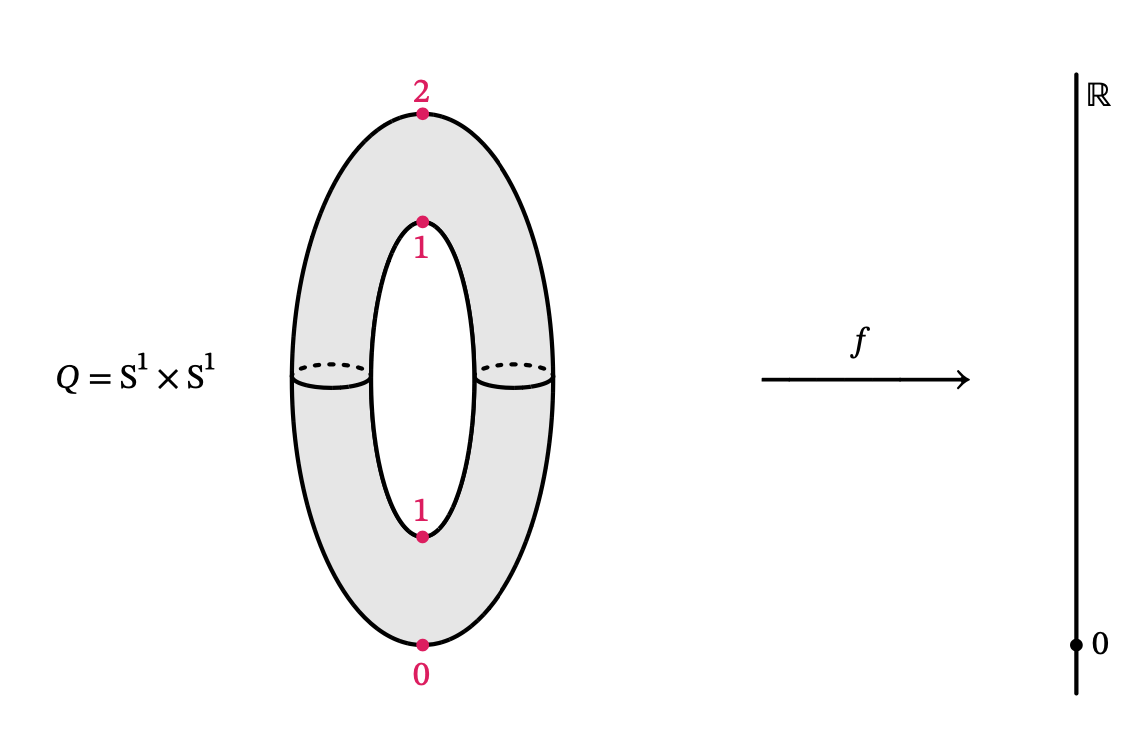
\includegraphics[width=9.3cm]{images/Lecture on Morse Theory/TORUS MORSE THEORY.png}
\end{center}
 Here we have 4 special points: the top and bottom, and then the two points in the middle. What happens in these points is that the shape of the preimage changes:
\begin{itemize}
    \item the preimage of the top (and bottom) is a point
    \item the preimage of points between the top and middle point is a circle
    \item the preimage of the middle points is a wedge of circles
    \item the preimage of points between the middle points is a disjoint union of circles.
\end{itemize}
Note that at the special points the preimage is generally not a smooth manifold. These "special" points are critical points of $f$:
%TODO add what the strategy is

\begin{defn}[Critical point and critical value]
    Let $M$ be a closed $n$-manifold and $f:M\to\R$ a smooth map. A critical point of $f$ is a point $p \in M$ such that $(df)_p: T_p M \to T_{f(p)} \R \cong \R$ is \textit{not} surjective. 
    A critical value is the image of a critical point.
\end{defn}

\noindent So a critical point is a point of $M$ with tangent bundle ``vertical'' with respect to $\R$ (thinking of $f$ as some kind of projection).

The main goal then is to recover (up to diffeomorphism) $M$ from knowing the critical points and the behaviour in a neighborhood thereof. 


\noindent Firstly we can define what we mean by a ``nice'' function:
\begin{defn}
    A Morse function is a smooth map $f: M \to \R$ such that all critical points are nondegenerate, that is if $p$ is a critical point of $f$, then 
    $\Hess(f)_p := \left( \frac{\de^2 f}{\de x_i \de x_j}(p)\right)_{i,j}$
    is non-singular (i.e. $\text{det}(\Hess(f)_p)\neq 0$).
\end{defn}
\begin{rem}
    This is independent of the choice of chart. 
\end{rem}

\begin{ex}
    Let's start with a nonexample: the parabolic cylinder.
    %DRAWING
    \noindent With coordinates $x_1, x_2$, the Morse function drawn can be written as $f(x_1, x_2) = -x_1^2$.
    \noindent Then at every critical point the Hessian is given by
    \begin{equation}
        \Hess(f)_p = \begin{pmatrix}
            -2 & 0 \\
            0 & 0 
        \end{pmatrix}   
    \end{equation}
    which is clearly singular.

    \noindent Another nonexample is given by the function $f(x) = x^3$. Consider the map that goes from the graph of $f$ to its $y$ coordinate. Again the Hessian is singular at the critical point.
\end{ex}

%other example $f(x_1, x_2) = -x_1^2 -x_2^2$
% hessian is -2 0, 0 -2, two negative eigenvalues -> index -2

\noindent We're then interested in the local picture at a critical point.

\begin{defn}[Index of a critical point]
    If $p \in M$ is a nondegenerate critical point of $f : M \to \R$, the index of $f$ at $p$ is 
    \begin{equation}
        \ind_f (p) = \text{index of }\Hess(f)_p = \# \text{ negative eigenvalues of} \Hess(f)_p .
    \end{equation}
\end{defn}

\begin{ex}\label{ex:quadric}
    Consider the following basic examples: %DRAWINGS
    \begin{itemize}
        \item $f(x_1, x_2) = -x_1^2-x_2^2$, this has critical point $p=(0,0)$ and there the Hessian is given by
        $\begin{pmatrix}
            -2 & 0 \\
            0 & -2 
        \end{pmatrix}$. We therefore see that $p$ is nondegenerate and that $\ind_f (p) = 2$.
        \item $f(x_1, x_2) = -x_1^2+x_2^2$, very similar, but $\ind_f (p) = 1$,
        \item $f(x_1, x_2) = +x_1^2-x_2^2$, again $\ind_f (p) = 1$,
        \item $f(x_1, x_2) = +x_1^2+x_2^2$, now $\ind_f (p) = 0$.
    \end{itemize}
\end{ex}

\noindent The examples above are very important, because locally Morse functions are always of one of those forms.
\begin{lem}[Morse Lemma I]
    Let $p \in M^n$ be a nondegenerate critical point of $f: M^n \to \R$ of index $k$. Then there is a chart $(U, \phi)$ around $p$ such that the map $\tilde f$ defined as
    \begin{equation}
        \begin{tikzcd}
            U \ar[r, "\phi"] \ar[d, "f"]& \R^n \ar[dl, "\tilde f"] \\
            \R
        \end{tikzcd}
    \end{equation}
    is given by:
    \begin{equation}
        \tilde f (x_1, \dots, x_n) = f(p) - \sum_{i=1}^k x_i^2 + \sum_{j=k+1}^n x_j^2
    \end{equation}
\end{lem}

\begin{proof}[Idea of proof]
    Given a nondenerate critical point of index $k$ we only know that $\Hess(f)_p$ has $k$ negative eigenvalues, is nonsingular and is diagonalizable. That allows me to change the basis so that the function takes that form, essentially doing a Taylor expansion. In particular then the chart can be chosen such that the function is \textit{exactly} that expression.
\end{proof}

% -------------------------------------------------------------
% --------------------- LECTURE 6 13/11 -----------------------
% -------------------------------------------------------------

\noindent Given a Morse function $f: M \to \R$, $p \in M$, then we have the following immediate consequences of the lemma:
\begin{itemize}
    \item if $p$ is critical ( and nondegenerate since is a \textit{Morse} function), because of the lemma we have a chart as above. Then the level sets $f^{-1} (f(p))$ look like a neighborhood of 0 in a quadric (locally).
    \item if $p$ is regular (that is, non-singular), by the implicit function theorem there are coordinates such that $f(x_1, \dots, x_n) = x_1$. So the level sets $f^{-1} (f(p))$ look like a submanifold in $\R^n$ (locally).
\end{itemize}
This explains what we noticed initially for the example of the torus, that the level set changes when passing a critical point. In particular it always changes in one of the ways shown in \ref{ex:quadric}. This observation will be more complete after Morse Lemma II and Theorem \ref{thm:handle_attachment_morse} below.

The following theorem justifies the use of Morse theory to study manifolds.
\begin{thm}
    For any manifold Morse functions exist.
    \label{thm:morse_exist}
\end{thm}
\noindent It's not trivial but it can be proven with tools from differential topology.

Example of something we can prove with Morse functions:
\begin{thm}
    The Euler characteristic can be calculated by knowning the critical points and the corresponding indices of a Morse function:
    \begin{equation}
        \chi(M) = \sum (-1)^k c_k
    \end{equation}
    where $c_k$ is the number of critical points of index $k$.
\end{thm}
\noindent This is quite clear for the sphere and the genus $g$ surfaces with the usual Morse functions, but it's interesting that for \textit{any} Morse function we have this result.

The following theorem also seems very plausible from the drawings:
\begin{lem}[Morse Lemma II]
    Let $f: M \to \R$ be a Morse function, $a< b \in \R$ such that $f$ does not have a critical value in $[a,b]$. Then
    \begin{equation}
        M_a = f^{-1} ((-\infty, a]) \hookrightarrow M_b = f^{-1} ((-\infty, b])
    \end{equation}
    is a (smooth) deformation retract. In particular, it induces a diffeomorphism $f^{-1}(a) \cong f^{-1}(b)$.
\end{lem}
\noindent Concretely this tells us that the level set \textit{only} changes when crossing a critical point.
\begin{rem}
    The proof uses flow along vector field $\frac{\grad f}{|\grad f|}$... %DRAWING...
\end{rem}

We will restrict to the following class of Morse functions:
\begin{defn}[Admissibile Morse function]
    A Morse function $f: M \to [a,b]$ is admissibile if $\de M = f^{-1}(a) \cup f^{-1}(b)$ and $a,b$ are regular values.
\end{defn}
% but can I have im f = [a,c] with c<b and f^-1 (c) = emptyset?
\noindent The fact that they're regular values is important, since it gives us that a neighborhood of $f^{-1}(a)$ is diffeomorphic to a cylinder $f^{-1}(a) \times [0, \epsilon]$, i.e. a collar (and the same is true for a neighborhood of $f^{-1}(b)$). So an admissible Morse function naturally equips $M$ with the structure of a cobordism from $f^{-1}(a)$ to $f^{-1}(b)$.

\noindent Another useful theorem, analogous to \ref{thm:morse_exist} is the following:
\begin{thm}
    Admissible Morse functions exist.
\end{thm}
%TODO add reference to Kosinski Differentiable manifolds.

%tells us how the level set changes before and after the critical point
We would now like to know \textit{how} the level set changes before and after the critical point. In order to do this we first introduce the concept of handle attachment.
\begin{defn}[Handle attachment]
    Let $M^n$ be an $n$-manifold and let $H^j \coloneqq D^j \times D^{n-j}$ for $j=0,1,\dots, n$. In addition let $f: \de D^j \times D^{n-j} \hookrightarrow \de M^n$ be an embedding and note that $\de D^j \times D^{n-j}$ also embeds into $H^j$. We can then \textit{attach a j-handle} to $M^n$ by gluing along $f$ to obtain the manifold 
    $M^n \amalg_f H^j$.
\end{defn}
\noindent This concept will be studied in one of the exercises. The following claim makes the definition meaningful:
\begin{clm}
    $M^n \amalg_f H^j$ has a smooth structure.
\end{clm}
\noindent Since we're interested in 2 manifolds, let's make explicit what it means to attach a $j$ handle to a 2 manifold:
\begin{itemize}%DRAWINGS
    \item $j=0, H^0 = D^0 \times D^2\cong D^2$ and we attach along the empty set (since $\de D^0 = \emptyset$), i.e. we take the disjoint union with $D^2$.
    \item $j=1, H^1 = D^1 \times D^1$ and we attach along $\de D^1 \times D^1$, i.e. along two segments
    \item $j=2, H^2 = D^2 \times D^0$ and we attach along $\de D^2 \times D^0\cong S^1$, i.e. along a circle
\end{itemize}
\noindent We can now see how the level sets change at a critical point.
\begin{thm}[\cite{Hirsch1976} Theorem 3.2, p.157]
\label{thm:handle_attachment_morse}
    Let $M^n$ be compact and $f: M^n \to [a,b]$ an admissible Morse function. Suppose that $f$ has a unique critical point $z$ of index $j$.

    \noindent There is an embedding $\iota: D^j \hookrightarrow M^n$ with image $e^j :=  \im \iota$ (called "belt disk"), satisfying: 
    \begin{itemize}
        \item $z \in e^j$;
        \item $e^j \subset M^n \setminus f^{-1}(b)$;
        \item $f^{-1}(a) \cap e^j = \de e^j = \iota (\de D^j)$, this is also called "belt sphere";
        \item $M$ deformation retracts onto $f^{-1}(a) \cup e^j$.
    \end{itemize}
    The embedding can then be extended to $e^j \times D^{n-j}=: H^j$.
    %DRAWINGS
    We can now choose an $a'$ with $a<a'< f(z)$ and we then have
    \begin{equation}
        M^n \cong f^{-1}([a,a']) \cup_{\bbar \iota} H^j
    \end{equation}
    (for $n=2$ this is a unique diffeomorphism up to isotopy\footnote{See \ref{Isotopy} for the definition of isotopy.}).
\end{thm}
\noindent This theorem explains what happens to the level sets when we meet a critical point of index $j$: we attach a $j$ handle! 
To use the terms above: we extend the belt disk to a $j$ handle and attach it to the boundary by gluing along the belt sphere (which is also extended).
Of course, all the drawings presented are for 2 manifolds and we will only apply these results to such manifolds, but this theorem works more in general! 

\begin{ex}
\hfill%TODO not very clear
    \begin{itemize}
        \item index 0: $M=S^2$ % DRAWING
        we then have $e^0 = \{z\}$, $\iota: D^0={pt} \hookrightarrow M$ and $\bbar \iota: D^0 \times D^2 \hookrightarrow M$.
        \item Now what happens when attaching a 1-handle $\im \bbar \iota$? %DRAWING
        Chose: $D^{n-k} \hookrightarrow \de (S^1 \times [0,1] \amalg S^1 \times [0,1])$
        \item Start with $S^1 \times [0,1]$. Want to attach a 1-handle $D^1 \times D^1$. %DRAWING
        But now we can attach in two ways. With a simple band or with a twisted one.
        \item Let's start again with a cylinder and attach a 2-handle $D^2 \times D^0$, so I kind of close one of the two side of the cylinder. %DRAWING
        We see that the 1-handle and the 2-handle kind of cancel each other out!
        \item Analogously, starting with a disk and attaching a 0-handle and then a 1-handle, these also cancel each other out!
    \end{itemize}
\end{ex}

\begin{prop}[VI 7.1 in \cite{kosinski2013differential}, "Handle slides"]
    If $\tilde M := (M \coprod_f H^j) \coprod_g H^i$ and $i\leq j$, then $\tilde M$ can be obtained by first attaching $H^i$ and then $H^j$.
\end{prop}
\noindent Note that the word \textit{can} in the proposition is important: if we were to simply commute the two attachments $(M \coprod_g H^i) \coprod_f H^j$ we would get something that in general doesn't make sense, since the map $g$ goes into $M \coprod_f H^j$, not just $M$, and $H^i$ may no longer be attached at the boundary, leading to a space that is not even a manifold. The proposition instead says that there exist maps $\tilde g$ and $\tilde f$, into $M$ and $M \coprod_{\tilde g} H^i$ respectively, such that $(M \coprod_f H^j) \coprod_g H^i \cong (M \coprod_{\tilde g} H^i) \coprod_{\tilde f} H^j$.
\begin{ex} %DRAWING
\hfill
    \begin{itemize}
        \item $j=1, i=0$ 
        \item $j=2, i=1$ same picture but upside down!
        \item $j=i=1$ do it as an exercise.
    \end{itemize}
\end{ex}

\noindent What happens if $i>j$? In general it's not so simple, but if $i=j+1$ the following result holds.
\begin{prop}[VI 7.4 in \cite{kosinski2013differential}, "Handle cancellation"]
    Let $\tilde M := (M \coprod_f H^j) \coprod_g H^{j+1}$, where the attaching sphere of $H^{j+1}$ intersects the belt sphere of $H^j$ "transversely" in one point. Then $\tilde M \cong M$.
    %attaching sphere defined p 105 Kosinski but i don't understand how it's different from the belt sphere
\end{prop}
%Need M different from emptyset right??
\begin{ex}
    $j=0$ %DRAWING
\end{ex}


% -------------------------------------------------------------
% --------------------- LECTURE 7 15/11 -----------------------
% -------------------------------------------------------------

\begin{thm}[\cite{Hirsch1976} 8.3.4, p. 187]
    Let $M$ be a surface admitting a Morse function that has exactly two critical points. Then
    \begin{equation}
        M \cong S^2
    \end{equation}
\end{thm}
\begin{rem}
    In dimension 1,2 and 3 all the homeomorphic manifolds are also diffeomorphic. 
\end{rem}
\begin{proof}
    Because of the remark it's enough to prove the homeomorphism, rather than the diffeomorphism.

    \noindent Assume $p_+, p_- \in M$ are critical points. Since $M$ is compact, also $f(M)$ is compact and therefore has a maximum and a minimum, which exactly correspond to the two critical points. Now assume $p_+$ is the maximum, then $\ind p_+ = 2$. Now, because of Morse Lemma I we have $\exists U_+$ a neighborhood of $p_+$ with coordinates $x_1, x_2$ such that 
    \begin{equation}
        f|_{U_+} = -x_1^2 - x_2^2 + f(p_+)
    \end{equation}
    %DRAWING
    Then we have $\exists b < f(p_+)$ such that $D_+ = f^{-1}([b, +\infty)) \cong D^2$.

    \noindent Similarly, $\exists U_-$ a neighborhood of $p_-$ with coordinates $x_1, x_2$ such that 
    \begin{equation}
        f|_{U_-} = x_1^2 + x_2^2 + f(p_-)
    \end{equation}
    and now we have $\exists a > f(p_-)$ such that $D_- = f^{-1}((-\infty,a]) \cong D^2$.

    \noindent Let $B_+, B_-$ be disjoint caps around the poles of $S^2$ and denote $C := S^2 \operatorname{int} (B_+ \amalg B_-) \cong S^1 \times [0,1]$. % there was f,x star but I didn't understand TODO
    Now, notice $\de D_+ \cong S^1 \cong \de D_-$ and we have a diffeomorphism $h_0: D_+ \to B_+$ as they are both diffeomorphic to $D^2$. In addition $h_0 |_{\de D_+} \de D_+ \to \de B_+$.
    Notice that between $[a,b]$ there are no critical values, that is $f^{-1}([a,b])$ has no crtiical points
    Now, using Morse Lemma II we get:
    \begin{itemize}
        \item $f^{-1}((-\infty, b]) =: M_b \hookrightarrow M_a :=f^{-1}((-\infty, a])$, $f^{-1}(a) \cong f^{-1}(b)$
        \item $f^{-1}([a,b]) \cong f^{-1}(a) \times [0,1] \cong S^1 \times [0,1] $% again f,x star TODO
    \end{itemize}
    Now we can extend $h_0|_{\de D_+}$ to $h_1: \de D_+ \times [0,1] \to \de B_+ \times [0,1]$. Now we can glue $h_0$ and $h_1$
    \begin{equation}
        h: D_+ \cup (\de D_+ \times [0,1]) \to B_+ \cup (\de B_+ \times [0,1]) % TODO add what the two are isomorphic to
    \end{equation}
    \begin{clm}
        If $g: S^1 \to S^1$ is a homeomorphism, then it can be extended to a homeomorphism $\tilde g: D^2 \to D^2$.
    \end{clm}
    \noindent $\tilde g$ can simply be defined as follows
    \begin{equation}
        \tilde g(x) = 
        \begin{cases}
            ||x|| g\left(\frac{x}{||x||}\right), & \text{for } x\neq 0\\
            0, & \text{for } x=0
        \end{cases}
    \end{equation}
    From the claim $h$ can be extended to a homeomorphism $M \to S^2$.
\end{proof}

\begin{rem}
\hfill
    \begin{enumerate}
        \item For any closed $n$ manifold that has two critical points, we have $M \cong S^n$ (\textit{homeomorphic}, not \textit{diffeomorphic}).
        \item (From Milnor) There are manifolds $M$ homeomorphic to a sphere but not diffeomorphic (e.g. $S^7$), we then talk about \textit{exotic spheres}.
    \end{enumerate}
\end{rem}

\begin{thm}[Classification of surfaces]\label{Classification of 2d manifolds}
    Let $M^2$ be an oriented, connected, closed surface. Then it can be obtained as in the following drawing:
    %DRAWING
\end{thm}

% -------------------------------------------------------------
% --------------------- LECTURE 8 20/11 -----------------------
% -------------------------------------------------------------

\begin{proof}
$ $ \newline  % to go to a new line after the word proof
    \indent Step 1: Choose an admissible Morse function $f$.
    
    Step 2a: If necessary, "perturb" $f$ to get distinct critical values. %DRAWING

    Step 2b: Chop into pieces with exactly one critical point and apply Morse Lemma I. We then get that $f^{-1}((-\infty, a_i])$ is obtained from $f^{-1}((-\infty,a_{i-1}])$ by attaching a handle.

    Goal: normal form (for closed connected surfaces) %DRAWING to explain from what to what we're going
    %why are copants still attaching a one handle??

    Step 3: Claim: We can obtain $M$ by first attaching 0-handles, then 1-handles, $\dots$, in ascending order.

    To prove this there are two strategies:
    \begin{enumerate}
        \item Use proposition about handle cancellation (first attaching $i$ handle and then $i+1$ handle these cancel) and handle slides: %DRAWING
        with these you can write down an algorithm to get the normal form from any handle decomposition.
        \item One can change the Morse function. Claim: We can choose $f$ such that if $\ind p_1 < \ind p_2 \implies f(p_1) < f(p_2)$. %DRAWING
        This can be proven by changing the Morse function locally around a critical point (see \cite{Hirsch1976} for more details). %TODO add ref
    \end{enumerate}

    Step 4: If $\de M = \emptyset$, then either $M = \emptyset$ or I have at least two critical points.

    \noindent Case 1: We have exactly 2 critical points which gives us $M \cong S^2$ because of Lemma. %TODO add ref

    \noindent Case 2: If we have $>2$ critical points, look at minimum, then there exist a neighborhood $D_-$ of the minimum such that $D_- \cong D^2$, i.e. a 0 handle attached to $\emptyset$ (because of Morse Lemma I $f$ locally looks like a cup).

    \noindent Starting from the minimum, attach one 0-handle. If then we attach another 0-handle, then we can use the handle slides and cancellations to get rid of all 0 handles but one.

    \noindent Next we can attach one handles and we have two options, %DRAWING
    only one of which gives an orientable manifold.

    \noindent At "end", same argument as for why only one 0-handle read backwards shows that we only have one 2-handle (for example change $f$ to $-f$).

    \noindent This ends the proof.
\end{proof}

Question: What about the unoriented case? (\textit{Hint: enough to have one attachment of Möbius strip})

We now consider the case with boundary:
\begin{thm}[Classification of surfaces with boundary]
    Let $M^2$ be an oriented, connected surface. Then it can be obtained as in the following drawing:
    %DRAWING
\end{thm}
\begin{proof}
    Now $ \de M \neq \emptyset$, then $\de M = S^1 \amalg \dots \amalg S^1$. If $f$ is an admissible Morse function $f$ onto $[a,b]$ with $f^{-1}(a) \cong (S^1)^{\amalg m}$ and $f^{-1}(b) \cong (S^1)^{\amalg n}$. Now one can prove that we need neither 0-handles (if $m \neq 0$) nor 2-handles (if $n \neq 0$).
\end{proof}